\section{The Variable Eddington Factor}
\label{sec:fld_vef}

In the two previous sections, diffusion theories have been derived for the two extreme limits of transport. That is purely isotropic radiance, which happens in the limit of thick, highly scattering media or a delta distribution, which in turn happens in the limit of very transparent, low order scattering media. This section will introduce the variable Eddington Factor, which has its origins in the astrophysics domain (Brunner~\cite{Brunner02}). It serves as a conceptual framework in which flux-limited diffusion is embedded. While diffusive transport has been related to a diffusion equation, streaming transport has been shown to relate to advection. The Variable Eddington Factor allows for realizing and mixing both types of transport within a domain.
\begin{figure}[h]
\centering
%\missingfigure{show advection and diffusion transport}
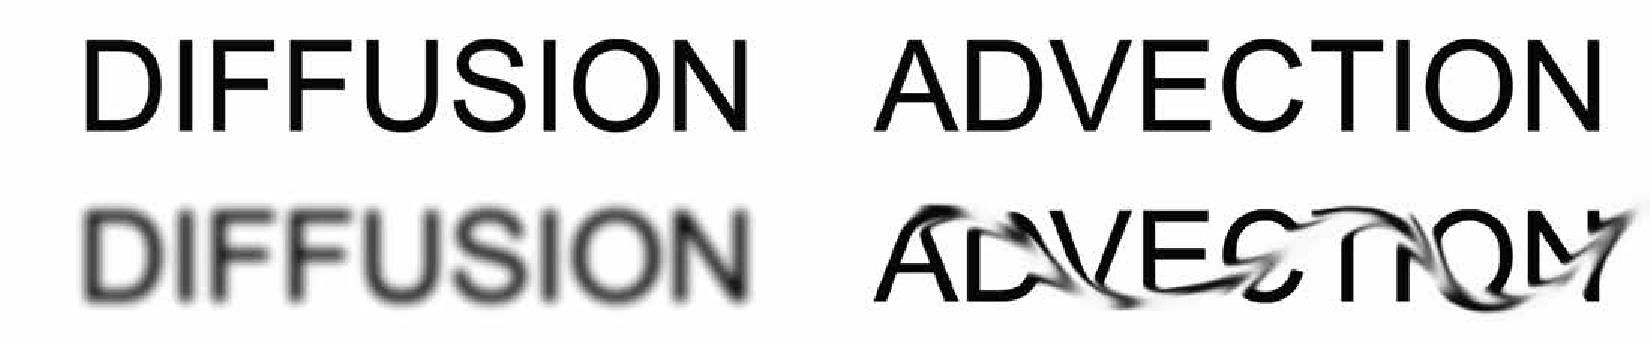
\includegraphics[width=0.95\textwidth]{06_fld/figures/fig_diffusion_vs_advection.pdf}
\caption{Illustration of diffusive (left) and advective (right) transport of particles. With diffusion, particles spread locally depending on the gradient of the particle distribution, which for flux-limited diffusion is the zero moment, the fluence. Advection is the movement of particles along a directed force field. For flux-limited diffusion, this force field is defined by the first moment, the flux vector.}
\label{fig:fld_vef_advection_diffusion}
\end{figure}


Classical diffusion assumed an isotropic distribution of radiance for the second moment, while pure streaming transport assumed a delta distribution. The Variable Eddington Factor theory assumes a radiance distribution, which is rotationally symmetric around a dominant vector $\vec{n}$. This assumption allows deriving a form for $T$, which represents isotropic distribution as well as a pure delta distribution and those forms inbetween, which are rotationally symmetric around a dominant direction $\vec{x}$.
\begin{figure}[h]
\centering
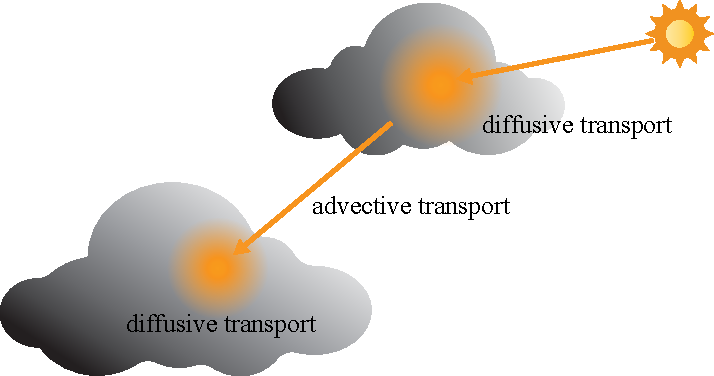
\includegraphics[width=0.55\textwidth]{06_fld/figures/fig_transport_regimes_scene.pdf}
%\missingfigure{show image with isotropic distribution, streaming limit distribution and inbetween forms}
\caption{Radiative transfer in typical scenes contains a mix of transport regimes as shown in this figure. Diffuse transport in dense media with high absorption and advective transport in thin media. The idea behind the Variable Eddington Factor is to express radiative transfer as a mix between those two extreme transport modes.}
\label{fig:fld_vef_advection_diffusion2}
\end{figure}

The Variable Eddington Factor form of $T$ is derived by considering a principal direction of transport, given by the vector $\vec{n}$ of unit length. An important assumption is that the radiance distribution will be radially symmetric around this direction. This means, that the value of $\hat{L}$ will be invariant to rotation about axis $\vec{n}$. It follows, that its first and second moment $\hat{L}_1$ and $\hat{L}_2$ will also be invariant to rotation about $\vec{n}$. If one approximates $\hat{L}_2$ using the Eddington tensor $T$ with $\hat{L}_2\approx T\phi$, it can be concluded that $\vec{n}$ will be an eigenvector of $T$ with eigenvalue $\chi$:
\begin{align*}
T\vec{n} = \chi\vec{n}
\end{align*}
%\TD{explain/give reference why eigenvectors need to sum up to one}
The plane perpendicular to $\vec{n}$ is an eigenspace of $T$. By requiring that all eigenvalues sum up to one, the eigenvalues of the two eigenvectors spanning that plane by distributing the remaining eigenvalue $1-\chi$ evenly between both is expressed as:
\begin{align}
\frac{1}{2}\left(1-\chi\right)\mathbf{I}
\label{eq:iso_var_T_isoterm}
\end{align}
From the free streaming limit case (section~\ref{sec:fld_streaming_limit_approximation}), it is known that $\chi=1$, when the radiance distribution becomes a delta distribution (equation~\ref{eq:zero_moment_Lhat} and~\ref{eq:first_moment_Lhat}). In that case, the eigenvalues associated with the eigenvectors perpendicular to $\vec{n}$ become zero and the term above vanishes.

Tensor diagonalization allows for explicitly adding the eigenvector $\vec{n}$ to the matrix by adding $\vec{n}_i\vec{n}_j$ (with $\vec{n}$ being of unit length). The scaling of its coefficients is found by considering that the term in equation~\ref{eq:iso_var_T_isoterm} introduces three eigenvectors. The sum of their eigenvalues will be $3/2(1-\chi)$. Since eigenvalues of the final tensor $T$ need to add up to one, the eigenvalue associated with the matrix $\vec{n}_i\vec{n}_j$ will be $\left(1- \frac{3}{2}\left(1 - \chi\right)\right)$. This results in the following form for $T$:
\begin{align}
T &= \frac{1}{2}\left(1-\chi\right)\mathbf{I} + \left(1- \frac{3}{2}\left(1 - \chi\right)\right) \vec{n}\otimes\vec{n}
\nonumber
\\
&= \frac{1}{2}\left(1-\chi\right)\mathbf{I} + \frac{1}{2}\left(3\chi-1\right) \vec{n}\otimes\vec{n}
\label{eq:iso_var_T}
\end{align}
This form of $T$ is called the Variable Eddington Tensor (VET). It can be understood as an \emph{interpolation} between an isotropic distribution tensor ($1/3\mathbf{I}$) and a delta distribution tensor ($\vec{n}_i\vec{n}_j$). The variable $1/3 \le \chi \le 1$ is the interpolation variable and is called the variable Eddington factor (VEF). Theories, which respect this structure of the Eddington tensor are referred to as theories under the variable Eddington factor formalism (VEF-formalism).

If $\chi=1/3$, then equation~\ref{eq:iso_var_T} will result in the isotropic distribution tensor, which is the base assumption for classical diffusion:
\begin{align}
\frac{1}{2}\frac{2}{3}\mathbf{I} + \frac{1}{2}\left(\frac{3}{3}-1\right) \vec{n}\otimes\vec{n}
=\frac{1}{3}\mathbf{I} + 0\vec{n}\otimes\vec{n} = \frac{1}{3}\mathbf{I}
\end{align}
For $\chi=1$, equation~\ref{eq:iso_var_T} produces the Eddington tensor, which was derived for the pure streaming limit distribution, where all light comes from a singular direction:
\begin{align}
\frac{1}{2}0\mathbf{I} + \vec{n}\otimes\vec{n}
= \vec{n}\otimes\vec{n}
\end{align}
The Eddington factor $\chi$ can also be interpreted as a measure of anisotropy of the radiance distribution $\widehat{L}$ with respect to direction $\vec{n}$. It can be expressed in terms of the radiance distribution by the squared mean cosine (given by Levermore~\cite{Levermore84}):
\begin{align}
\chi &= \int_{S^2}{ \left(\vec{\omega}\cdot\vec{n}\right)^2\hat{L}\left(\vec{x}, \vec{\omega}\right)\ud\vec{\omega}}
\label{eq:iso_var_chi}
\end{align}
With the variable Eddington factor approach, only a function for the interpolation variable $\chi$ (the actual Eddington factor) needs to be identified. This function should have $1/3$ and $1$ as its limits. With such an interpolation function, the limit transport cases (diffusion and free streaming) will be a subset of any theory, which adheres to the variable Eddington factor concept.

The Eddington factor framework, sets up the Eddington factor and the limits of its parameterization, $\chi$. The specific expression for this factor is not defined and it is clear that there are many options for the function $\chi$, which respect the given function limits. This is why there is such a rich variety of theories in other domains, which all propose their own version of that interpolation function. Some of them are ad-hoc schemes (Bowers et al.~\cite{Bowers82}, Kershaw~\cite{Kershaw76} and Larsen et al.~\cite{Larsen74}), which are derived from heuristics, while others have a clear connection to transport theory (Levermore at al.~\cite{Levermore81}) or are derived from entropy theory (Minerbo~\cite{Minerbo78}).

The general strategy for all these different variable Eddington factor theories is:
\begin{enumerate}
\item Find a model or theory, from which a certain radially symmetric form of the radiance distribution $\hat{L}$ about the normalized flux-vector$\vec{E}/\phi$ can be found or justified.
\item Then derive an expression for $\chi(\vec{E}/\phi)$ from the model for $\hat{L}$, which can be used to construct $T$. Further assumptions are applied, to be able to express $\vec{E}$ in terms of $\nabla\phi$. This is required in order to not have $T$ depend on the flux-vector directly as it still needs to be possible to resolve equation~\ref{eq:me_first_resolved_E} for the flux-vector.
\end{enumerate}

In this thesis, results for different theories have been presented and implemented, but only flux-limited diffusion from Levermore et. al~\cite{Levermore81} was discussed, since it is the most popular and also has the strongest connection to transport theory. Discussing all other theories is beyond the scope of this thesis and also not really necessary, as it is shown in section~\ref{sec:fld_results} that the particular choice of theory is not of significant importance for applications in computer graphics.